
To analyze a huge amount of images requires a better way of handling and sorting them than just storing them into directories. A set of scripts where built arround a database to let us create trainging and testing sets easilier. Borrowing ideas on how is the transfer learning process made by the engineers in the tensorflow team, our catalog system grew to answer to these needs. In a later stage the analysis process was also included into the system spawning what could become a framework to analyze visual patterns in sets of images with many different purposes.\\

The development process showed the need of a better set of tools to overcome several difficulties that were found. The training stage involved a repetitive process consisting of manually inspecting the available imagery. To this end, a web application was built on top of our catalog system facilitating this process. The process of continuously showing and tagging images proved to be error prone, each mistakenly tagged picture, required to log into the database and delete the wrong entry after maching encoded file names. So a new feature was implemented into our tool, it shows the stored images and their respective tag and lets the user either delete or edit the classification. Finally, when the model was already trained and it was predicting on the orthorectified rasters, the ability to geolocate the predicted damaged areas and place them in a map was very convenient.\\

As it was just exposed, the application was built thinking about the end user. Even though the correct implementation from a design perspective is out of the scope of this work, it was an interesting thing to explore as this would be the kind of problems to be solved in the case of getting such a system into production. The last few paragraphs explained how the system grew to a full server-client architecture to respond to the need of processing data and visualizing the results in a meaningful way.\\

The purpose of this chapter, is to talk about the implementation of our experiment. Details of the pipeline architecture, and the techniques used to obtain and curate data are unveiled.\\

\section{Backend}

To understand why some design decision where made we need to understand the nature of our data. Data came in directories taken from the drones and splitted by flying dates. The quantity and naming of the images was not uniform across towns. Additionaly, drone imagery provide metadata that is useful to geolocate the images. However, this information is limited as it only offers the place where the image was taken but gives no information about the image resolution. This difficulty is overcome with specialized software that takes in the set of images and creates a mosaic using the images using a process known as orthorectification which corrects the distortions caused by the angle in which the image was taken. CENAPRED gave us both resources, the raw drone images and the ortorectified rasters. So the first part of the application was to transform these data into a way that would be easier to manage.\\

Given to previous experience in developing similar projects, it was decided that the system was to be built on top of a Python Web framework. It offers many solutions out of the box, including a familiar line interface set of commands and an object relational mapper that makes the database integration easier. The feature of being ready to offer a web interface was a great plus.\\

\subsection{Data model}

We took advantage of the object relation mapper system that Django offers. In the figure \cite{fig:database} we show a subset of the database diagram. Tables inherent to the features of the Django framework are not shown as they where not modified.\\

The database design was based on reproducible reaseach. We wanted to keep track of the charactistics of the models trained. Also we wanted to know which where the training images used for each model. It was also desirable to be able to reuse models that where trained with different sets of images to benchmark and finally use the best model to actually predict on the orthorectified raster.\\


In order for the tagging application to work, images must be ingested into the system so every time a new sample is tagged we populate the database with information about the original image and the coordinates relative to the original image. In the final stage of the process we produce a list of potential damaged buildings which are also inserted into the database with geografical information and human readable address. We think that this can be helpfull to allocate resources in the most efficient way.\\

\begin{figure}[h]
  \begin{center}
    \subfigure{\label{fig:database}\fbox{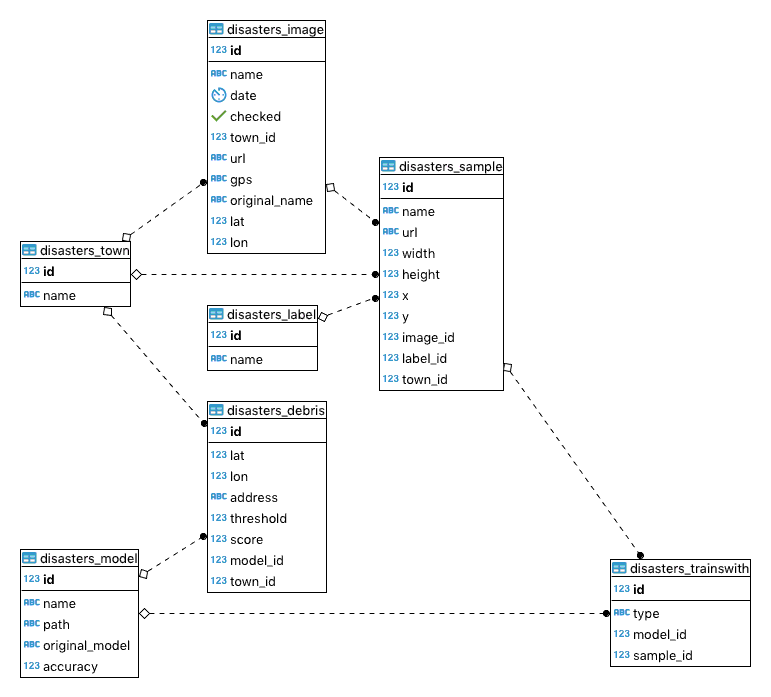
\includegraphics[width=1\textwidth]{images/database.png}}}
  \end{center}
\end{figure}

We built a system to ingest the images from the NOAA service. It lazily downloads the images by checking first if the file is already present in the temporary folder. If the file does not exist it downloads it, then the system tries to add it to the database and persistent file system. To maintain a coherent one to one mapping between the database and the file system, the process of adding a new scene must be successful both in the database and in the filesystem, otherwise, the file is erased from both, and the state of the system remains as it was before the ingestion attempt.\\

\subsection{Tag}


Aerial tagged data is scarce. In particular, for the purpose of our experiment, we don't have any useful metadata on the images. We propose a method to tag samples of the scenes using crowd sourcing. We built a service that crops samples from the images and exposes them to an online application that lets any user with access to tag an image. We have three categories: the image has water in it, the image does not have water in it, and it is not possible to tell. When a positive answer is obtained, the system persists de image in the data base with the information of from which scene was it extracted.\\


\section{Data augmentation}

Given the nature of our task, it is hard to acquire the tagged images. To increment the size of our training dataset, even more, we use a technique known as data augmentation. It relies on the fact that affine transformations do not change the content of the scenes, however, a transformed scene appears as a completely new one to the classifier.\\

The images were rotated by 10 degrees, and reflected by the x-axis and the y-axis this gives us a $x144$ factor, this means that for each tagged image, the training corpus is incremented by $144$ images. The problem with this approach is that when a square image is rotated, some information on the corners is lost so we have to adjust the original image so that we can still crop a complete square from the desired size from it. For our experiment, the input size for the neural network is $227\times 227$ pixels, so the original images must be at least $\sqrt{2}$ times $227$ on each side. This way no matter how we rotate the original image, we can still crop a $227\times 227$ from the center of the rotation without losing any data.\\



\section{Train}

We needed data to train our model. Raw dron images where obtained from the National Center for Disaster Prevention (CENAPRED). Drons flew over three towns in the state of Oaxaca producing $3733$ images during several days. Images contain gps information about the place where they where taken, however, it is not posible to produce a one to one mapping from the pictures to georeferenced points. With this limitation it was not possible to locate possible damaged buildings from the raw images. However, the model does not need any geografical information to be trained as it relies only in the pixel intensities.

Cropping and tagging manualy a large number of samples from the images was prohibitive. In order to overcome this obstacle an online tagging application was developed for this purpose. The idea was to decentralize the tagging procedure by giving an easy to use tool that was able to run from any browser. This way the cumbersome task of tagging the images can be crowdsourced.

By consuming the REST api described in the previous section, a simple web client was developed using jquery and openlayers. The interface is an image viewer with a selection and a button to submit an opition on that the higlighted area. The user will select an appropiate section of the given image, tag it, and then submit the section. In the backend, the image is cropped and ingested into the database.

\begin{figure}[h]
  \begin{center}
    \subfigure{\label{fig:database}\fbox{\includegraphics[width=1\textwidth]{images/visualise.png}}}
  \end{center}
\end{figure}

An additional button is given that lets the user see how well is the current best model performing. The process is quite similar to the previous one. In the server, the image is cropped and then the thumbnail is exposed to the model and the result is written back to the client through the REST api.

\begin{figure}[h]
  \begin{center}
    \subfigure{\label{fig:database}\fbox{\includegraphics[width=1\textwidth]{images/predict.png}}}
  \end{center}
\end{figure}


\begin{figure}[h]
  \begin{center}
    \subfigure{\label{fig:database}\fbox{\includegraphics[width=1\textwidth]{images/submit.png}}}
  \end{center}
\end{figure}

During the process, we noticed that the tagging process can lead to errors. In order to deal with those mistaken tagged images, a visualiser for the tagged images was developed. It consist in a simple interface where the last tagged images are shown with their respective tag. The interface offers a way to delete a given image or just edit the previously assigned tag.

\begin{figure}[h]
  \begin{center}
    \subfigure{\label{fig:database}\fbox{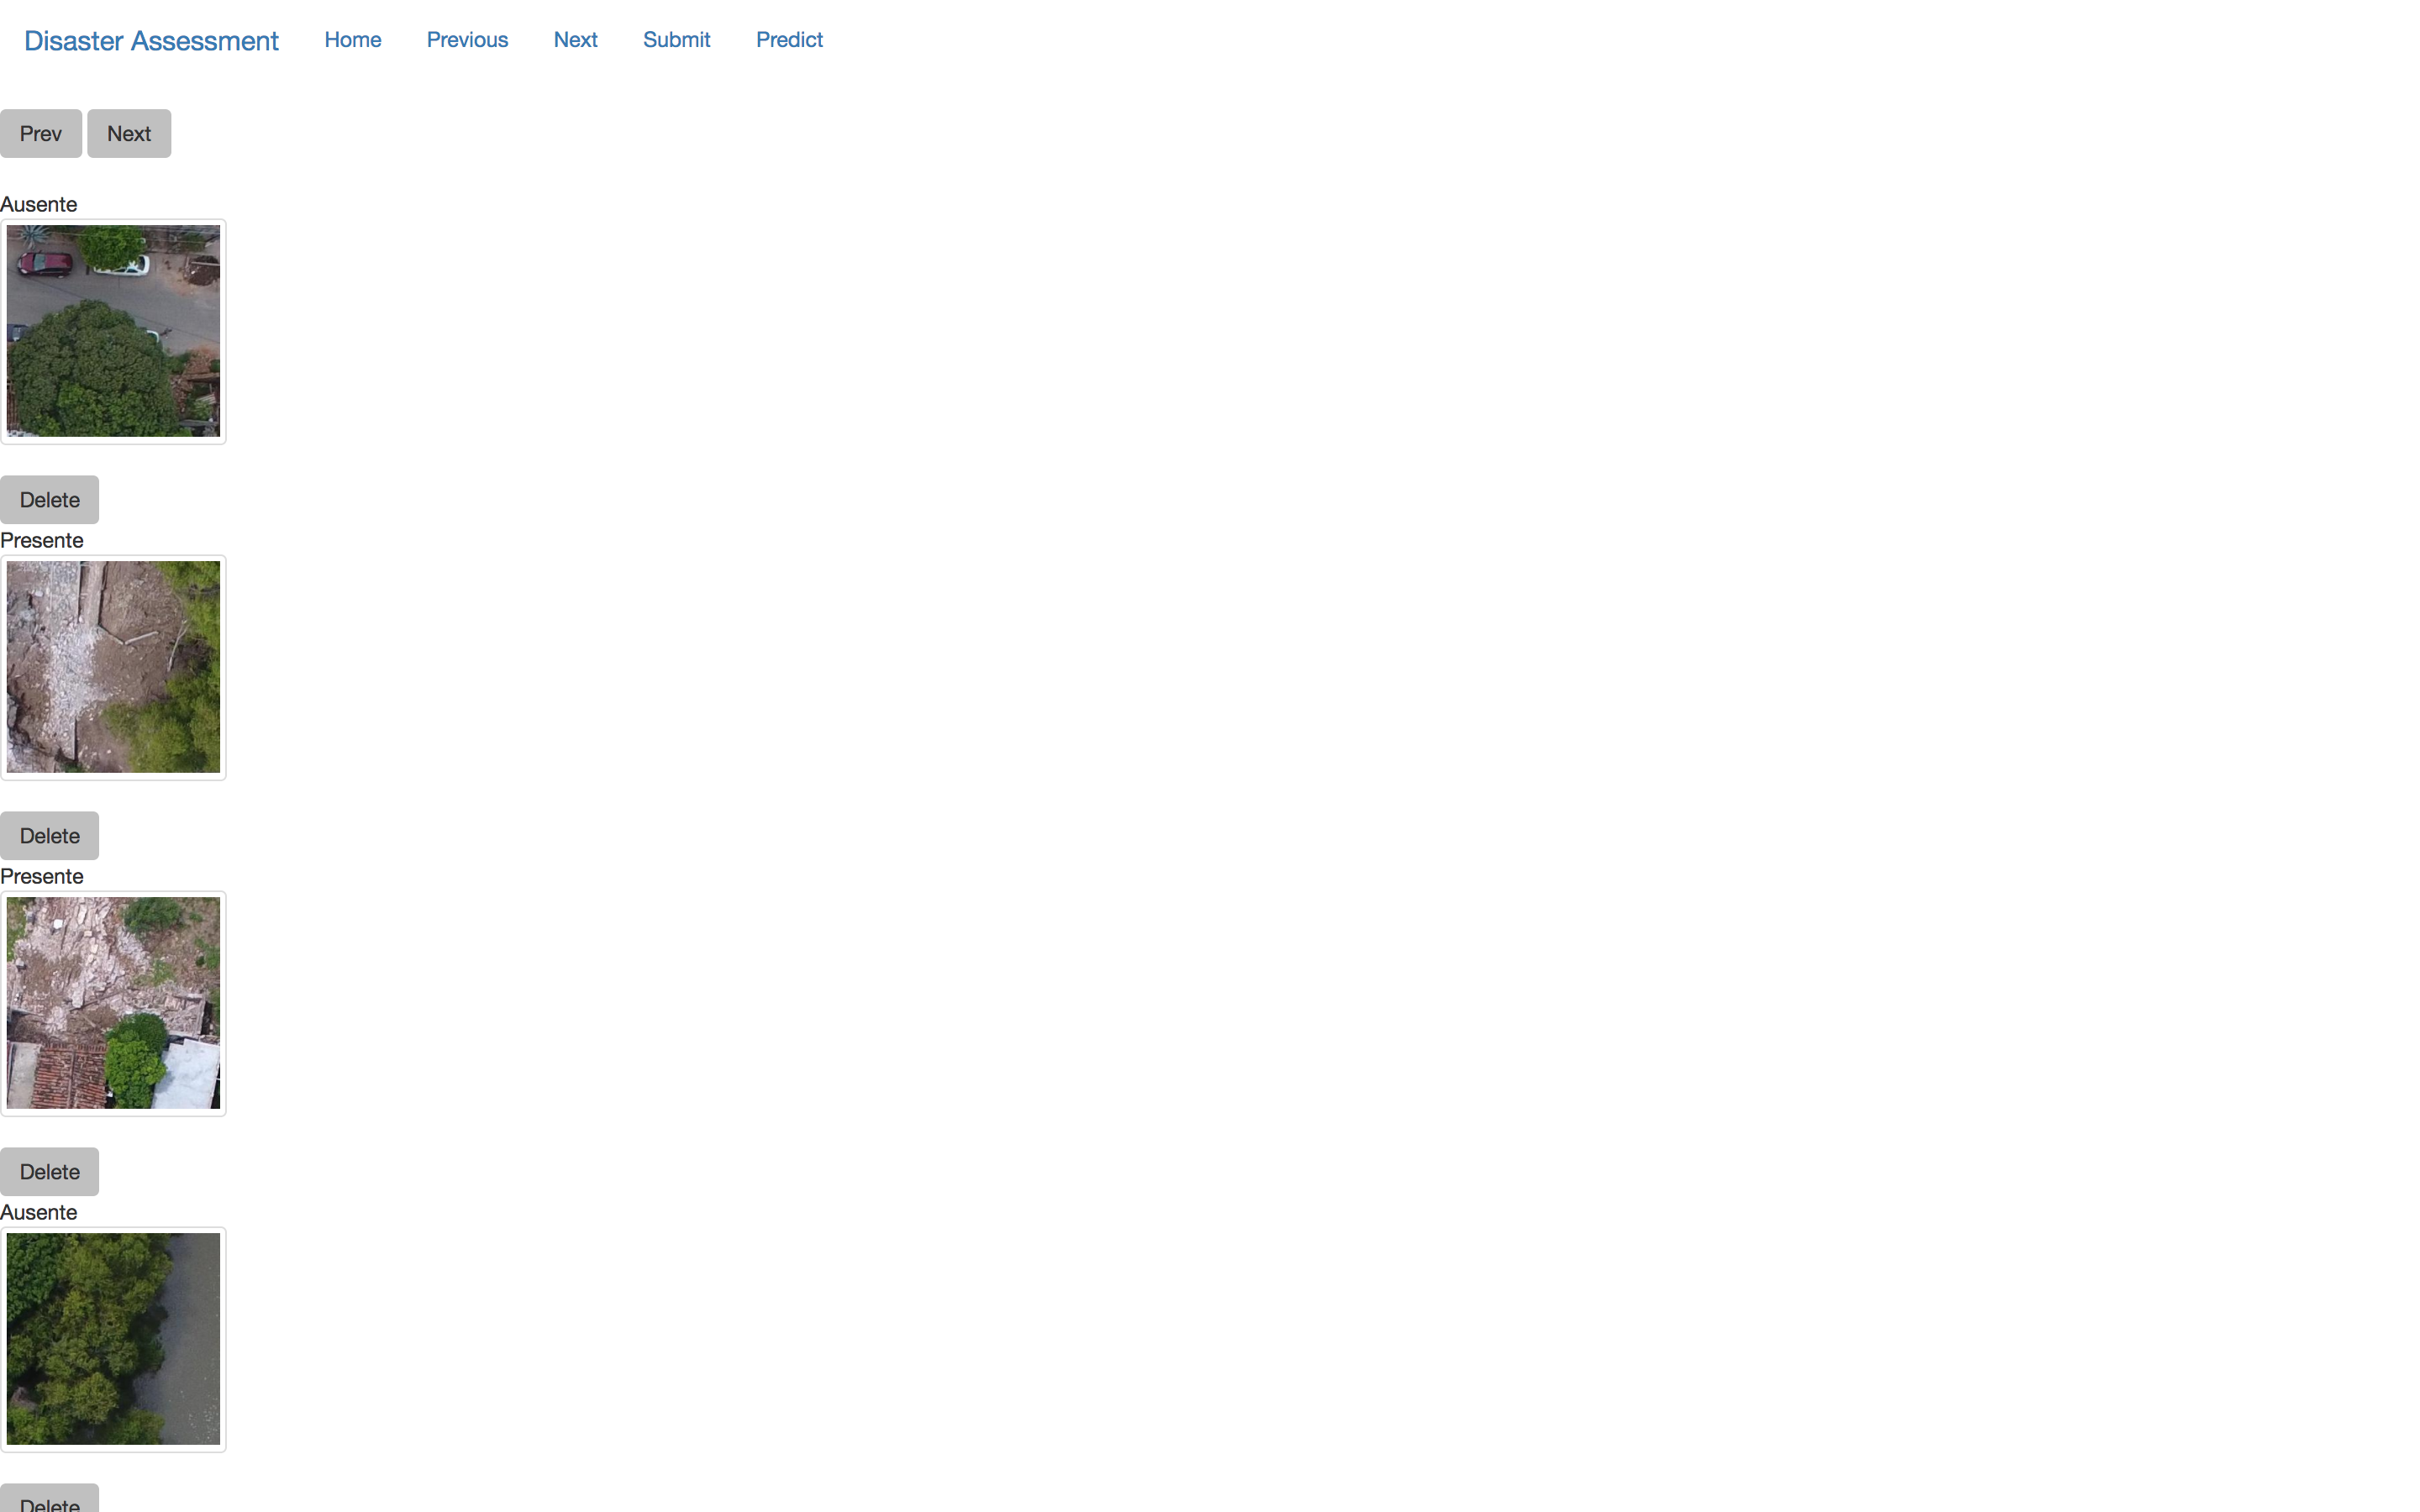
\includegraphics[width=1\textwidth]{images/thumbnails.png}}}
  \end{center}
\end{figure}
Finally, we developed a view for the points that the algorithm finds in the ortorectified image. This view was implemented with open layers and shows information about the location of the potential damaged building in a human readable form. This is done by querying the google api with the latitude and longitude points extracted from the map.

\begin{figure}[h]
  \begin{center}
    \subfigure{\label{fig:database}\fbox{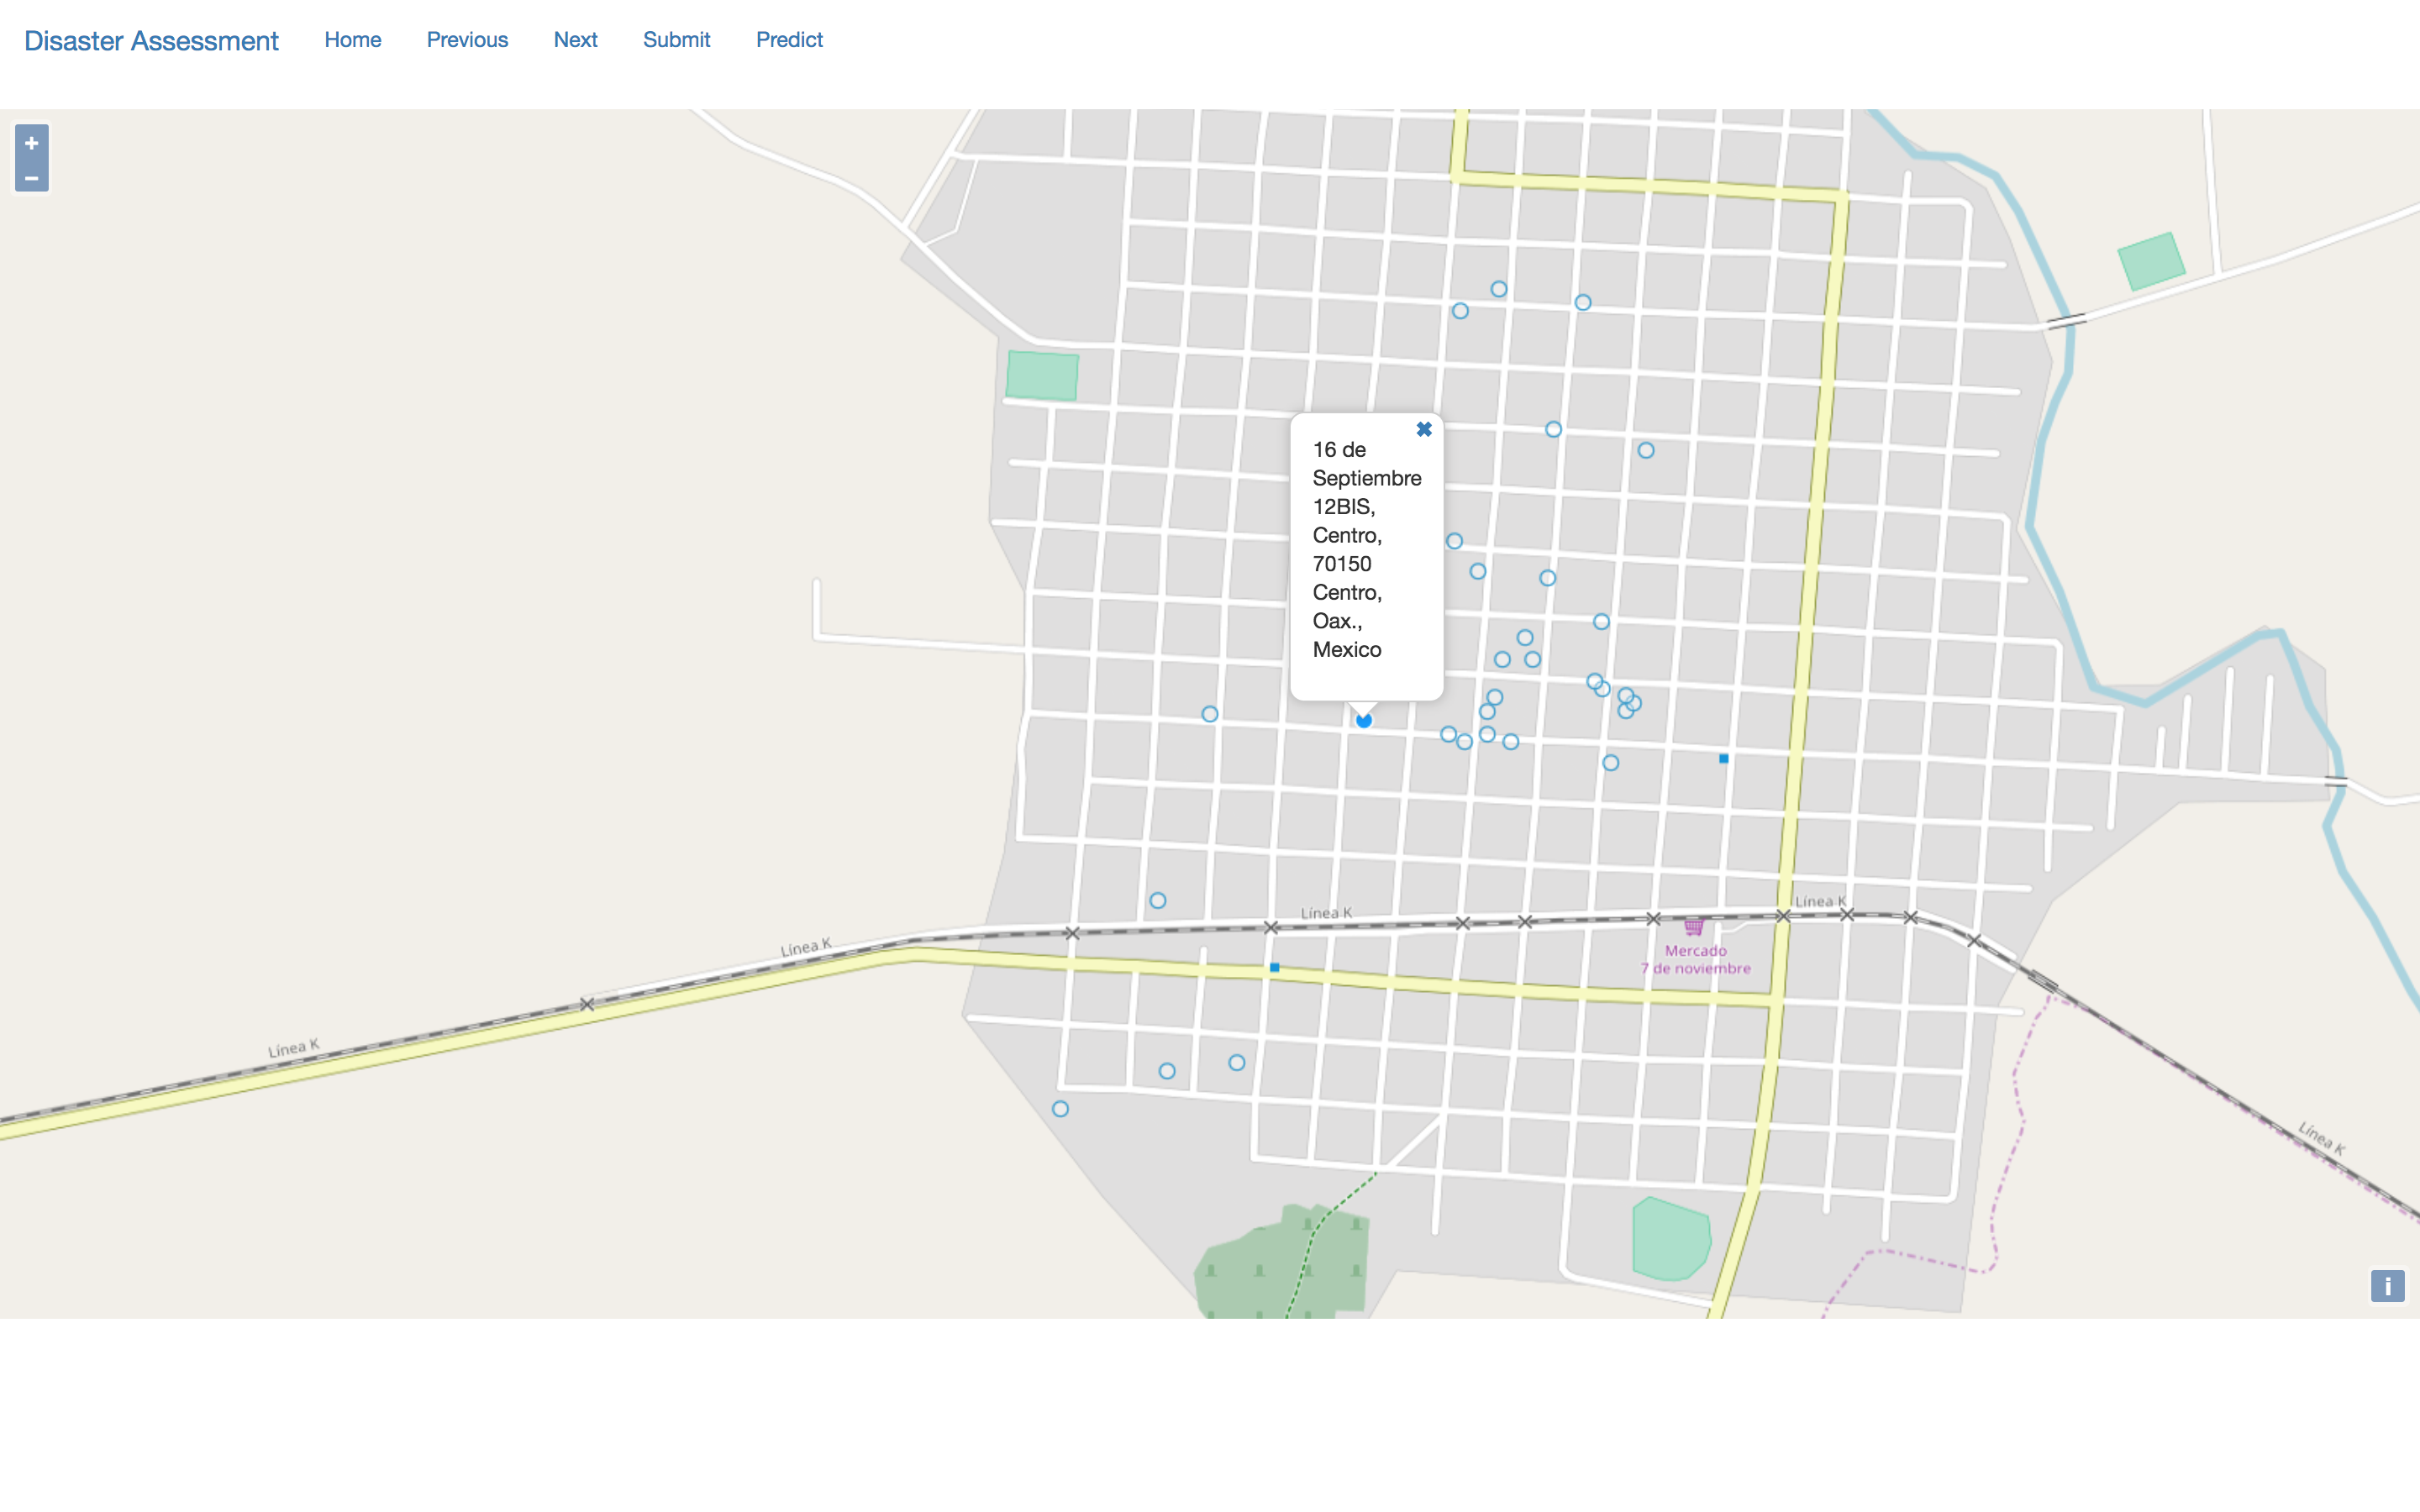
\includegraphics[width=1\textwidth]{images/debris.png}}}
  \end{center}
\end{figure}

\section{Predict}

Another simple front end application was developed to predict on new features, it is very similar to the tagging application. Instead of asking the user about the correct tag, it queries the model and exposes the answer to the front end.\\



\section{Model creation}

In order to create the model we need to select a sample from the thumbnails that we extracted from the original images. We wanted to create a process that was easily reproductible so we would compare models in a simple fashion. To this end the sample must be random each run and we need to split the images in three sets: training, validation and testing.\\

Tensorflow provides a script to retrain the last layer of inception by conecting the extracted features into a sofmax layer, and then training this classifier on the given set. It requires a directory layout tailored built to this purpose. The script was modified to fit our database design in order to make as easy as possible to train several models with homogeneous training, validation, and testing sets.


